% Latex Beamer Template
%
% Copyright 2010 by Frederik Beuth (beuth@hrz.tu-chemnitz.de) - TU-Chemnitz, Dep. for CS, Professorship Artificial Intelligence
%
% Your are allowed to use the latex beamer class and the structure of this latex template for your presentation.
% This template contains a complete presentation from me. This is intended to demonstrate to you the different features of Latex Beamer.
% Your are NOT allowed to use the content of template for your presentations, hence the presented ideas of this template belongs still to me.
%
% Usage: use pdflatex
%
\documentclass[12]{beamer}
\mode<presentation>
{
  \usetheme{AIChemnitz}
  \setbeamercovered{transparent}
	% bei Schrittweisem aufdecken sind die noch nicht gezeigten Punkte
	% nur blass dargestellt (nicht ausgeblendet)
}

\usepackage[USenglish]{babel} % localized output
%\usepackage[latin1]{inputenc} % Input encoding (you can directly use special chars) for windows
\usepackage[utf8]{inputenc} % or for UTF-8 (linux)
\usepackage[T1]{fontenc}    % use Umlaute directly
%\usepackage{times}         % if you want use the times font
\usepackage{textpos}        % to use an absolute position for figures => figure[H]

%if you want to use pdslatex=>dvi=>ps=>pdf 
%\usepackage[dvips]{graphicx}
%load packages without options as latest
\usepackage{
	calc,			% extend of the arithmetic functions
	color,			% to switch in the running text simple with \color{Farbe) with Farbe = e.g.red, blue, black etc.
				% or use \textcolor{farbe){Text)
	fancybox,		% shadowbox, doublebox, ovalbox, Ovalbox 
	fancyvrb,		% verbatim extension
	float,			% to use absolut positions of the 'figure'- or 'table'-environment 
				% with figure[H]
	mdwlist,		% compact list: itemize* ..
	tabularx,		% table with variable column width
%own packages
	lscape,
	amsmath,		%for extended math
	bm,			%for bold math fonts
	xspace,			%spaces in macros are not ignored with xspace
	subfigure		%for sub figures
}

%this directory will be automatic searched for graphics
\graphicspath{{./images/}}

% This part display the outline at the begin of each section
% if unintended, simply comment this out
\AtBeginSubsection[]
{
  \begin{frame}<beamer>
    \frametitle{Gliederung}
    \tableofcontents[currentsection,currentsubsection]
  \end{frame}
}

%
% basis information about the presentation
%
\title{TITEL}
\subtitle{~} % Subtitel, use ~ if you want an empty subtitle
\author{Frederik Beuth, Fred. H. Hamker}
%\date{\today}
\date{21/10/2010} %the date of the presentation
\occasion{KI2010} %the occasion

\linespread{1.15} %line spread (currently 110% )


%
% examples of different New-Commands
% 
\newcommand{\zb}{z.\,B.~}
\newcommand{\equates}{\mathrel{\widehat{=}}}
%define the displaying of the neuronal area name for equations
\newcommand{\Area}[1]{^{\mbox{\tiny #1}}}

%Example of a new-command with 2 parameters, e.g.
%\subtexGrafic{0.5}{Overview.jpg} shows the grafic 'Overview.jpg' as 50% of the text width
%#1 => variable for the first parameter, #2 => for the second parameter
\newcommand{\subtexGrafic}[2]{
	\subfigure[#2]{\label{fig:#1}\input{texImg/#1}}
}
%show a normal grafic
\newcommand{\showGrafic}[2]{
	\begin{center}
		\includegraphics[width=#2\textwidth]{#1}
	\end{center}
}


\begin{document}

% create title slide
\begin{frame}[plain]
  \titlepage
\end{frame}
%
\begin{frame}
  \frametitle{Outline}
  \tableofcontents
\end{frame}


\section{Goals}
\begin{frame}
  	\frametitle{Goals}
	\begin{itemize}
	  \item Enhance object recognition by neuro-computational concepts.
	  \item Concept of visual attention can solve the problem of parallel segmentation and recognition.	  
	  \item Combine the concept of attention with shape-based object recognition.
	  \item Use a stereoscopic input to be applicable to robots with two cameras.
	\end{itemize}	
\end{frame}


\section{Concept of visual attention}
%
\begin{frame}
  	\frametitle{Concept of attention - key ideas}
	\textbf{Concept of visual attention} (Hamker, 2005): \\
	Focus processing on a spatial part of the image or at a subset of features.

	\textbf{Key ideas:}
	\begin{enumerate}
	  \item Parallel processing over all hierarchical areas in the visual stream.
	  \item Selection of cells: first spatial, and second feature-based.
	\end{enumerate}	
\end{frame}

\begin{frame}
    \frametitle{Visual Cortex}
    \showGrafic{visualCortex5}{0.8}
\end{frame}

\begin{frame}
  	\frametitle{Parallel processing}	
	\showGrafic{parallelProcessing3}{0.9}
	\begin{itemize}
	  \item Bottom-up processing, driven by conspicuous image points like edges, corners, \ldots
	  \item Top-down processing, hence which object is expected.
	\end{itemize}
\end{frame}

\begin{frame}
  	\frametitle{Feature-based selection of cells}
	\showGrafic{featureSelection}{0.9}
\end{frame}

\begin{frame}
  	\frametitle{Information integration}
	\showGrafic{attention}{0.8}
	Activation $r_j$ for cell $j$:
        \begin{center}
	  $\tau \frac{\Delta r_j}{\Delta t} = (\sum_i w_{i,j} \cdot r_i ) \cdot (1+a_j-\max\{a\})$
	\end{center}
\end{frame}

\begin{frame}
	\frametitle{Spatial selection of cells}
	\showGrafic{spatialSelection}{0.9}
\end{frame}

		
\section{Model}
%
\begin{frame}
  \frametitle{Outline}
  \tableofcontents[currentsection]
\end{frame}

\begin{frame}
  \frametitle{Model}
 \begin{center}
    \vspace{0.5em}
  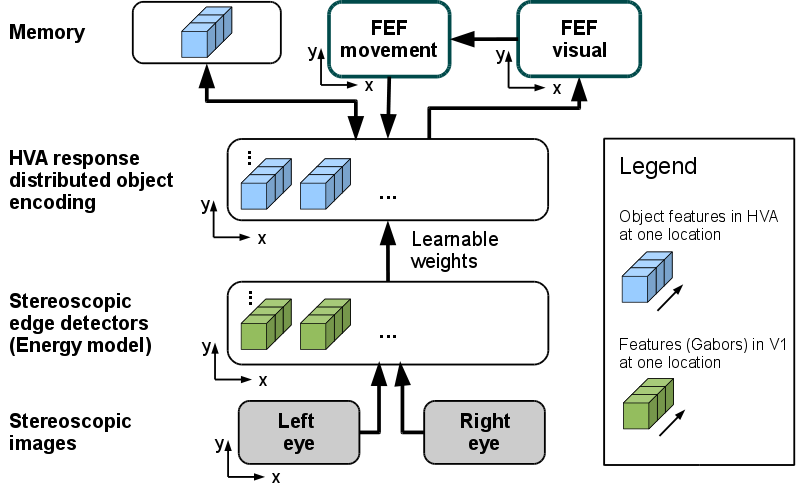
\includegraphics[width=0.9\textwidth]{overviewCore3}
\end{center}
\end{frame}

\begin{frame}
  \frametitle{Learning}
  \begin{itemize}
   \item Idea: A following image belong probably to the same object then the last image.
   \item Present a slowly in depth moving object as input.   
   \item Use a Oja like trace learning rule (simplified form):
      $$\tau \frac{\Delta w}{\Delta t} = r\Area{HVA} (trial-1) \cdot r\Area{V1}(trial) - \alpha \cdot (r\Area{HVA})^2 \cdot w $$
   \item Achieve view encoding cells with scaling and depth invariances.
  \end{itemize}
\end{frame}


\section{Results}

\begin{frame}
  \frametitle{Outline}
  \tableofcontents[currentsection]
\end{frame}

\begin{frame}
 	\frametitle{Temporal behavior}
	Experiment:
	\begin{enumerate}
	  \item Present an object alone and memorize it.
	  \item Search the object in a complex scene.
	\end{enumerate}
	\begin{figure}
	  \subfigure{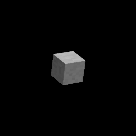
\includegraphics[width=0.17\textwidth]{2ob_03Target_L}} \quad \quad \quad \quad
	  \subfigure{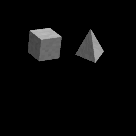
\includegraphics[width=0.17\textwidth]{2ob_03All_L}}
	\end{figure}
\end{frame}

\begin{frame}
 	\frametitle{Object recognition}
	Recognition of 10 different Objects:
	\showGrafic{objectsGray_b}{0.6}
	\begin{enumerate}
	  \item Present each object alone at a random position and memorize it.
	  \item Search and recognize the object in a complex scene.
	\end{enumerate}	
\end{frame}


\section{Summary}
%
\begin{frame}
  \frametitle{Outline}
  \tableofcontents[currentsection]
\end{frame}
%
\begin{frame}
  \frametitle<presentation>{Summary}
  % the summary should be very short
	\begin{itemize}
		\item Demonstrate the psychological concept of attention in connection with learned shape-based detectors.
		\item The concept will also work well with other descriptors.
		\item Model is able to recognize and localize an object in parallel.  	
	\end{itemize}
\end{frame}
%
\begin{frame}
 	\frametitle{Future work}
	\begin{itemize}
	  \item Area HVA is an abstraction of V2, V4 and TEO/TE.
	  \item The attention signal is not applied at V1.
	  \item The stereoscopic edge detector does not work with huge disparities.
	\end{itemize}
\end{frame}


%
\LARGE
\begin{frame}
	\frametitle{Acknowledgments}
	%if you want to display something at the last slide
	%\begin{figure}[H]
	%\vspace{1em}
	%	\begin{center}
	%		Questions?
	%	\end{center}
	%\vspace{3em}
	%\end{figure}

%if the work was founded by some grant (e.g.EU, BMBF or DFG-project)
\begin{figure}
      \subfigure{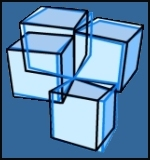
\includegraphics[width=0.15\textwidth]{eyeshotsLogo5}} 
      \subfigure{
\includegraphics[width=0.7\textwidth]{eyeshotsLogoBig}}
\end{figure}
\small
\begin{description}
  \item [Acknowledgments:] This work has been supported by the EC Project FP7-ICT ``Eyeshots: Heterogeneous 3-D Perception across Visual Fragments''.	
\end{description}

\end{frame}

\end{document}
